\section{Resource-Exception Model}
\label{sec:resexcmodel}

We next present our resource-exception model that describes expected behaviors after
exceptions occur while using resources such as database connections or files. In general,
a resource usage includes three actions: creation, manipulation, and cleanup. In our context, the cleanup
action not only includes closing the resource but also includes other actions such as 
rolling back of uncommitted transactions. Our resource-exception model primarily
captures the required cleanup action after exceptions occur during resource 
creation and manipulation actions. We next present the definitions for the three actions 
in the context of our approach through Scenario 1 in Figure~\ref{fig:threescenarios}.

\textbf{Resource Creation.} A resource-creation action represents method invocations
that create resources. For example, the method invocation \CodeIn{OracleDataSource}.\CodeIn{getConnection}
is an example resource-creation action. 

\textbf{Resource Manipulation.} A resource-manipulation action represents method invocations
that manipulate created resources. The method invocations in Lines 8-10 of Scenario 1 are examples of resource
manipulation actions. Sometimes, a resource-manipulation action can produce
new objects. In our context, we conservatively consider that method invocations on these newly created objects also
manipulate the original resource.

\textbf{Resource Cleanup.} A resource-cleanup action represents method invocations
that release created resources. The method invocations in Lines 12, 15, 16, and 17
are examples of resource-cleanup actions.

A resource-exception model from Scenario 1 is shown in Figure~\ref{fig:resourcemanip}.
We show normal and exception edges in solid and dotted lines, respectively. The model
shows the expected behaviors when exceptions occur after executing the resource-manipulation
action \CodeIn{Statement.executeUpdate}. Note that existing 
approaches such as Weimer and Necula~\cite{WeimerN05} mine rules 
that include resource-creation and resource-cleanup actions only. These rules
describe that the resource creation should be followed by the
resource cleanup in all paths including exception paths. However, 
a simple combination of resource creation and resource cleanup may not be
able to capture several scenarios that can help detect defects.
We explain the issue through Scenarios 1 and 2 shown in Figure~\ref{fig:threescenarios}.

Scenarios 1 and 2 show code examples where a \CodeIn{connection} resource is created through 
the resource-creation actions \CodeIn{OracleDataSource}.\CodeIn{getConnection}
and \CodeIn{DriverManager.getConnection}, respectively. Scenario 1
attempts to modify the contents of the database through the resource-manipulation
action \CodeIn{Statement.executeUpdate} (Line 9), whereas Scenario 2 attempts to read contents
of the database through the resource-manipulation action \CodeIn{Statement.executeQuery} (Line 6).
From the resource-exception model for Scenario 1 (shown in Figure~\ref{fig:resourcemanip}), we can infer
a resource-cleanup action as \CodeIn{Connection.rollback}. However,
this cleanup action does not apply to Scenario 2, where there are no modifications
to contents of the database. Therefore, the cleanup action \CodeIn{Connection.rollback}
is applicable \emph{only} when the resource manipulation action \CodeIn{Statement.executeQuery}
is taken into consideration, because this manipulation action is the triggering
action for that cleanup action. To address the preceding issue, our resource-exception 
model includes resource-manipulation actions 
that are transitively dependent on the resource-creation action.
In our resource-exception model, we call the normal path between 
a resource-creation action and resource-manipulation
action as a \emph{trigger} path. The model describes that the cleanup
actions \CodeIn{Connection.rollback}, \CodeIn{Statement.close}, and \CodeIn{Connection.close}
should be executed when an exception
occurs after the resource-manipulation action \CodeIn{Statement}.\CodeIn{executeUpdate}.

\begin{figure}[t]
\centering
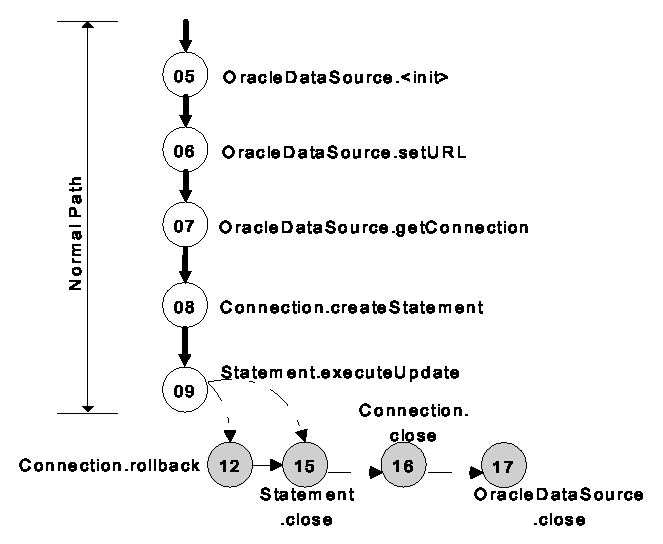
\includegraphics[scale=0.60,clip]{figs/approach-resexpmodel1.eps}\vspace*{-3ex}
\caption{\label{fig:resourcemanip} A resource-exception model} \vspace*{-4ex}
\end{figure}

We next describe the significance of a trigger path in our resource-exception model.
The primary rationale for considering the trigger path is that the same resource-manipulation
action can have different resource-cleanup actions based on different trigger paths.
Consider the same code example shown in Scenario 1 of Figure~\ref{fig:threescenarios}. Applying our
resource-exception model analysis, we can infer that a cleanup action for
the resource-manipulation action \CodeIn{Statement.executeUpdate} 
(Line 9) is \CodeIn{OracleDataSource.close} (Line 17).
However, such a cleanup action is not applicable to the resource-exception model
shown in Scenario 2 of Figure~\ref{fig:resourcemanip}. The primary reason is that the \CodeIn{connection}
resource is created through different resource-creation actions in Scenarios 1 and 2. Therefore,
considering the \emph{trigger} path helps distinguish the two scenarios.

